%\usepackage[usenames]{color}
%\mathscr{ABC} %Letra para F de fourier //No tomar la importante es la siguinte F
%%%%%%%%%%%%%%%%%%%%%%%%%%%%%%%%%%%%%%%%%%%						Hecho por Gris Cruces						%%%%%%%%%%%%%%%%%%%%%%%%%%%%%%%%%%%%%%%
%%%%%%%%%%%%%%%%%%%%%%%%%%%%%%%%%%%%%%%%%%%										ESCOM										%%%%%%%%%%%%%%%%%%%%%%%%%%%%%%%%%%%%%%%
%izq,der,arr,aba
%\newtheorem{thm}{Teorema} %Define Teoremas
%Demostraciones
%Definiciones
%$\mathcal{F}$ Transformada de Fourier


\documentclass[a4paper]{article}
%%%%%%%%%%%%%%%%%%%%%%%%%%%%%%%%%%%%%%%%%%%%%%%%%%%%%%%%%%%%%%%%%%%%%%%%%%%%%%%%%%%%%%%%%%%%%%%%%%%%%%%%%%%%%%%%%%%%%%%%%%%%%%%%%%%%%%%%%%%%%%%%%%%%%%%%%%%%%%%%%%%%%%%%%%%%%%%%%%%%%%%%%%%%%%%%%%%%%%%%%%%%%%%%%%%%%%%%%%%%%%%%%%%%%%%%%%%%%%%%%%%%%%%%%%%%
\usepackage[spanish]{babel}
\usepackage{graphicx}
\usepackage{anysize}

%TCIDATA{OutputFilter=Latex.dll}
%TCIDATA{Version=5.50.0.2953}
%TCIDATA{<META NAME="SaveForMode" CONTENT="1">}
%TCIDATA{BibliographyScheme=Manual}
%TCIDATA{LastRevised=Monday, March 05, 2012 08:31:36}
%TCIDATA{<META NAME="GraphicsSave" CONTENT="32">}

\marginsize{1.5cm}{1.5cm}{2.5cm}{1.9cm} 
\newtheorem{dmt}{Demostraci\'on}
\newtheorem {dfn}{Definici\'on}
\input{tcilatex}

\begin{document}

\tableofcontents
\listoffigures

%%%%%%%%%%%%%%%%%%%%%%%%%%%%%%%%%%%%%%%%%%%%%%%%%%%%%%%%%%%%%%%%%%%%%%%%%%%%%%%%%%%%%%%%%%%%%%%%%%%%%%%%%%%%%%%%%%%%%%%%%%%%%%%%%%%%%%%%%%%%%%%%%%%%
\begin{titlepage}
    \centering 
    	%\includegraphics[width=0.30\textwidth]{internet_11.jpg} \vspace{1cm} 

    \LARGE \textbf{Transformada de Fourier\\}
    	\rule{8.5cm}{2pt} \vspace{0.5cm}

    M. en C. Miguel Olvera Aldana\\

    \vspace{2cm} 

    M\'exico D.F.\\
    7 de Marzo de 2010
 \end{titlepage}
%%%%%%%%%%%%%%%%%%%%%%%%%%%%%%%%%%%%%%%%%%%%%%%%%%%%%%%%%%%%%%%%%%%%%%%%%%%%%%%%%%%%%%%%%%%%%%%%%%%%%%%%%%%%%%%%%%%%%%%%%%%%%%%%%%%%%%%%%%%%%%%%%%%%

\section{Introducci\'on}

\subsection{Clasificaci\'on de las Funciones}

\begin{dfn}
: Una funci\'on $f$ de un conjunto $D$ a un conjunto $E$ es un
correspondencia que asigna a cada elemento $x$ de $D$ un elemento \'unico de 
$E$. 
\end{dfn}

{} A veces se ilustran las correspondencias con diagramas como el de la
Figura~\ref{fig:correspondencia} en los que los conjuntos $D$ y $E$ quedan
representados por puntos dentro de ciertas regiones del plano. La flecha
indica que $y$ es elemento de $E$ que corresponden al elemento $x$ de $D$.
Lon conjuntos pueden tener elementos en com\'{u}n. De hecho muchas veces $D=E
$. 
\begin{figure}[h]
\centering
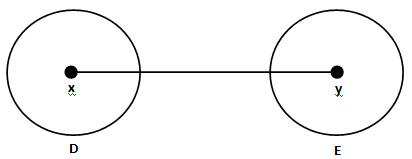
\includegraphics[width=0.40\textwidth]{f1p1.jpg}   
\caption{ {}}
\label{fig:correspondencia}
\end{figure}

{} La figura indica que a cada $x$ en $D$ le corresponde uno y solo un $y$
en $E$, es decir, dado $x$ se tiene que $y$ es \'unico. Sin embargo, a
varios elementos de $D$ les puede corresponder un mismo elemento de $E$. 

{} En general, $D$ y $E$ ser\'an conjuntos de n\'umeros. Por ejemplo, si $D$
y $E$ son conjunto de los n\'umeros reales, a cada numero real $x$ se le
puede asignar su cuadrado $x^{2}$. As\'i, a $3$ se le asigna $9$, a $-5$ se
le asigne $25$, a $5$ se le asigna $25$, y a $2$ se le asigna $4$, esto es
una correspondencia de correspondencia.

\subsubsection{Funciones Peri\'odicas, definici\'on y gr\'afica}

\begin{dfn}
: Un funci\'on $f$ se llama peri\'odica si esta definida para todo $t$ real
para alg\'un n\'umero positivo $T$, $f\left(t+T\right)=f\left(t\right)$ para
todo $T$. 
\end{dfn}

{} El n\'umero $T$ se llama el periodo de $f$. El periodo m\'inimo de $f$ se
llama periodo principal o periodo fundamental de $f$. Por ejemplo, $\sin
\left(t + 6PI\right) = \sin \left(t\right)$ para todo $t$. Por lo tanto $6PI$
es un periodo de la funci\'on seno. Sin embargo, el periodo principal de la
funci\'on seno es $2PI$ ya que $\sen \left(t + 2PI\right) = \sen %
\left(t\right)$ para todo $t$ y $2PI$ es el m\'inimo n\'umero con esta
propiedad. Geom\'etricamente esto significa que la gr\'afica de $f$ se
repite cuando las abscisas de los puntos toman valores en intervalos
sucesivos de amplitud $T$. La Figura~\ref{fig:seno1} muestra la funci\'on
peri\'odica con periodo $T$.  
\begin{figure}[h]
\centering
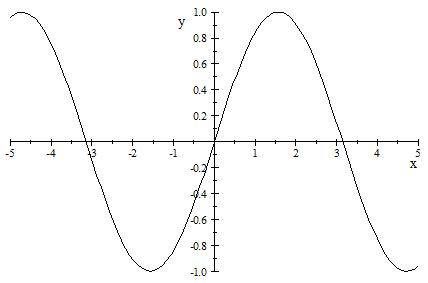
\includegraphics[width=0.40\textwidth]{f1p2.jpg}   
\caption{Funci\'on Peri\'odica}
\label{fig:seno1}
\end{figure}

\newpage 

\subsubsection{Funciones Pares e Impares, definici\'on y gr\'aficas}

\begin{dfn}
: Sea $f$ una funci\'on tal que siempre que $x$ este en el dominio $D$, $- x$
tambi\'en esta en $D$. 

\begin{itemize}
\item $f$ es par si $f\left(x\right)=f\left(-x\right)$ $\forall x \in D$. 

\item $f$ es impar si $f\left(-x\right)=-f\left(x\right)$ $\forall x \in D$. 
\end{itemize}
\end{dfn}

{} En la Figura~\ref{fig:coseno} se puede observar la gr\'afica del coseno
que es sim\'etrica con respecto al eje $y$, es decir, que tiene los mismos
valores en el eje $y$ para $\cos\left(x\right)$ que para $\cos\left(-x\right)
$  
\begin{figure}[h]
\centering
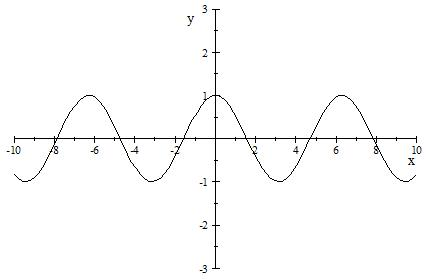
\includegraphics[width=0.40\textwidth]{f1p3.jpg}   
\caption{Funci\'on Par}
\label{fig:coseno}
\end{figure}

{} En la Figura~\ref{fig:seno} se puede observar la gr\'afica del seno que
es sim\'etrica respecto al origen, es decir, que tiene los mismo valores
para $\sin\left(-x\right)$ que para $-\sin\left(x\right)$  
\begin{figure}[h]
\centering
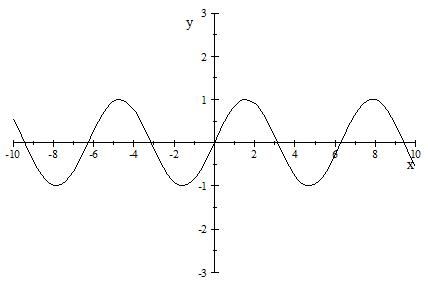
\includegraphics[width=0.40\textwidth]{f1p4.jpg}   
\caption{Funci\'on Impar}
\label{fig:seno}
\end{figure}
%%%%%%%%%%%%%%%%%%%%%%%%%%%%%%%%%%%%%%%%%%%%%%%%%%%%%%%%%%%%%%%%%%%%%%%%%%%%%%%%%%%%%%%%%%%%%%%%%%%%%%%%%%%%%%%%%%%%%%%%%%%%%%%%%%%%%%%%%%%%%%%%%%%%%

\section{Conceptos y definici\'on de Serie de Fourier}

{} Muchas funciones conocidas pueden desarrollarse en series infinitas e
integrales que contienen funciones trigonom\'etricas. Esta idea es
importante al modelar muchos fen\'omenos de la f\'isica, la ingenier\'ia, la
computaci\'on y la topograf\'ia asistida por computadora. 

{} Sea $f\left(t\right)$ una funci\'on peri\'odica con periodo $T$, la cual
puede representarse por una serie trigonom\'etrica.  
\[
f(t)=\frac{1}{2}a_{0}+a_{1}\cos (\omega_{0}t)+a_{2}\cos
(2\omega_{0}t)+a_{3}\cos (3\omega_{0}t) \ldots +b_{1}\sin
(\omega_{0}t)+b_{2}\sin (2\omega_{0}t)+b_{3}\sin (3\omega_{0}t)+ \ldots
\]

{} Entonces llamamos \textbf{Serie Trogonom\'etrica de Fourier} a la
siguiente expresi\'on.  
\[
f(t)=\frac{1}{2}a_{0}+\sum_{n=1}^{\infty}{\left(a_{n}\cos
(n\omega_{0}t)+b_{n}\sin (n\omega_{0}t)\right)}
\]

{} Una alternativa para la serie trigonom\'etrica de Fourier es:  
\[
f(t)=c_{0}+\sum_{n=1}^{\infty}\left(c_{n}(n\omega_{0}t-\theta n)\right)
\]

{} Donde los coeficientes $c_{n}$ y $\theta_{n}$ se conocen como las
amplitudes arm\'onicas y \'angulos de fase respectiva. 

\begin{dmt}
: 
\end{dmt}

{} Si tenemos que:  
\[
c_{n}=\sqrt{(a_{n})^{2}+(b_{n})^{2}} \hspace{4.2cm}
\]
\[
\cos (\alpha)=\frac{a_{n}}{\sqrt{(a_{n})^{2}+(b_{n})^{2}}} \hspace{3.5cm}
\]
\[
\sin (\alpha)=\frac{b_{n}}{\sqrt{(b_{n})^{2}+(b_{n})^{2}}} \hspace{3.5cm}
\]

{} Entonces:  
\[
a_{0}\cos (n\omega_{0}t)+b_{0}\sin (n\omega_{0}t)= \sqrt{%
(a_{n})^{2}+(b_{n})^{2}} \left(\frac{a_{n}}{\sqrt{(a_{n})^{2}+(b_{n})^{2}}}%
\cos (n\omega_{0}t) + \frac{b_{n}}{\sqrt{(b_{n})^{2}+(b_{n})^{2}}}\sin
(n\omega_{0}t)\right)
\]
\[
=c_{n}(\cos(\alpha)\cos(n\omega_{0}t)+\sin(\alpha)\sin(n\omega_{0}t)) 
\hspace{1.1cm}
\]
\[
=c_{n}(\cos(n\omega_{0}t-\alpha)) \hspace{4.3cm}
\]

{} Reescribiendo tenemos que:  
\[
\alpha=\theta_{n} \hspace{6.2cm}
\]
\[
\tan(\theta_{n})=\frac{b_{n}}{a_{n}} \hspace{0.2cm} \Rightarrow \hspace{0.2cm%
} \arctan \frac{b_{n}}{a_{n}}=\theta_{n} \hspace{2cm}
\]
\[
c_{0}=\frac{1}{2}a_{n} \hspace{5.9cm}
\]

{} Por lo tanto  
\[
f(t)=\frac{1}{2}a_{0}+\sum_{n=1}^{\infty}{\left(a_{n}\cos
(n\omega_{0}t)+b_{n}\sin (n\omega_{0}t)\right)} =
c_{0}+\sum_{n=1}^{\infty}\left(c_{n}(n\omega_{0}t-\theta n)\right)
\]

{} La expresi\'on para la serie de Fourier es una representaci\'on de
funciones peri\'odicas que se ve como la suma de componentes sinosoidales
que tienen diferentes frecuencias. La componente sinosoidal de frecuencia se
denomina la en\'esima frecuencia.  
\[
\omega_{n}=n\omega_{0}
\]

{} La primera arm\'onica se le conoce como la componente fundamental.  
\[
\omega_{0}=2\pi f \hspace{0.3cm} \Rightarrow \hspace{0.3cm} \omega_{0}=\frac{%
2\pi}{T}
\]

%%%%%%%%%%%%%%%%%%%%%%%%%%%%%%%%%%%%%%%%%%%%%%%%%%%%%%%%%%%%%%%%%%%%%%%%%%%%%%%%%%%%%%%%%%%%%%%%%%%%%%%%%%%%%%%%%%%%%%%%%%%%%%%%%%%%%%%%%%%%%%%%%%%%

\subsection{Funciones Ortogonales}

Un conjunto de funciones $\theta_{n}t$ es ortogonal en un intervalo $a<t<b$
si para cuales quiera de dos funciones $\theta_{n}t$ y $\theta_{m}t$ $\in$ $%
\theta_{v}t$ se cumple lo siguiente:  
\[
\int_{a}^{b}\theta_{n}(t)\theta_{m}(t)dt=0 \hspace{1cm} si \hspace{0.2cm}%
m\neq n
\]
\[
\int_{a}^{b}\theta_{n}(t)\theta_{m}(t)dt=r_{n} \hspace{0.9cm} si \hspace{%
0.2cm}m=n
\]
\newline

{} Consid\'erese el ejemplo de las funciones sinosoidales:  \newline

{} \textbf{\textit{a)}}  
\[
\int_{-\frac{T}{2}}^{\frac{T}{2}}\cos(n\omega_{0}t)dt=\left.\frac{1}{%
n\omega_{0}}\sin(n\omega_{0}t)\right|_{-\frac{T}{2}}^{\frac{T}{2}} \hspace{%
6.3cm}
\]
\[
=\frac{T}{2\pi n}\left[\sin \left(n\frac{2\pi}{T}\frac{T}{2}
\right)-\sin\left(n\frac{2\pi}{T}\left(-\frac{T}{2}\right) \right) \right]
\]
\[
=\frac{T}{2\pi n}(\sin(n\pi)+\sin(n\pi))=0 \hspace{2.2cm}
\]

{} \textbf{\textit{b)}}  
\[
\int_{-\frac{T}{2}}^{\frac{T}{2}}\sin(n\omega_{0}t)dt=\left.\frac{1}{%
n\omega_{0}}\cos(n\omega_{0}t)\right|_{-\frac{T}{2}}^{\frac{T}{2}} \hspace{%
6.5cm}
\]
\[
=\frac{T}{2\pi n}\left[-\cos \left(n\frac{2\pi}{T}\frac{T}{2}
\right)+\cos\left(n\frac{2\pi}{T}\left(-\frac{T}{2}\right) \right) \right]
\]
\[
=\frac{T}{2\pi n}(-\cos(n\pi)+\cos(n\pi))=0 \hspace{2.1cm}
\]

{} \textbf{\textit{c)}}  
\[
\int_{-\frac{T}{2}}^{\frac{T}{2}} \cos(n\omega_{0}t)\cos(m\omega_{0}t)dt 
\hspace{8cm}
\]

{} Si utilizamos las siguientes identidades trigonom\'etricas.  
\[
\cos(a+b)=\cos(a)\cos(b)-\sin(a)\sin(b)
\]
\[
\cos(a-b)=\cos(a)\cos(b)+\sin(a)\sin(b)
\]
\[
2\cos(a)\cos(b)=\cos(a+b)-\cos(a-b)
\]

{} Entonces:  
\[
\int_{-\frac{T}{2}}^{\frac{T}{2}} \cos(n\omega_{0}t)\cos(m\omega_{0}t)dt=
\int_{-\frac{T}{2}}^{\frac{T}{2}} \left[\frac{1}{2}\cos(n\omega_{0}t+m%
\omega_{0}t)+\frac{1}{2}\cos(n\omega_{0}t-m\omega_{0}t)\right]dt \hspace{4cm}
\]
\[
\hspace{0.4cm} = \frac{1}{2}\int_{-\frac{T}{2}}^{\frac{T}{2}%
}\cos((n+m)\omega_{0}t)dt+\frac{1}{2}\int_{-\frac{T}{2}}^{\frac{T}{2}%
}\cos((n-m)\omega_{0}t)dt
\]
\[
\hspace{1.8cm} =\frac{1}{2}\left[\frac{1}{(n+m)\omega_{0}}%
\sin((n+m)\omega_{0}t)+\frac{1}{(n-m)\omega_{0}}\sin((n-m)\omega_{0}t)\right]
\]
\[
\hspace{3.8cm} =\frac{1}{2}\left[\frac{T}{(n+m)2\pi}\sin \left((n+m)\frac{%
2\pi}{T}\frac{T}{2}\right) + \frac{T}{(n-m)2\pi}\sin \left((n-m)\frac{2\pi}{T%
}\left(-\frac{T}{2}\right)\right)\right]
\]

{} Si $m \neq n \neq 0$  
\[
\int_{-\frac{T}{2}}^{\frac{T}{2}} \cos(n\omega_{0}t)\cos(m\omega_{0}t)dt =%
\frac{1}{2}\left[\frac{T}{(n+m)2\pi}\left(\sin((n+m)\pi)-\sin(n+m)(-\pi)
\right)\right] \hspace{4.3cm}
\]
\[
\hspace{0.5cm} +\frac{1}{2}\left[\frac{T}{(n-m)2\pi}\left(\sin((n-m)\pi)-%
\sin(n-m)(-\pi) \right)\right]
\]
\[
=\frac{1}{2}\left[\frac{T}{(n+m)2\pi}(0+0)+\frac{T}{(n-m)2\pi}(0+0)\right] 
\hspace{1cm}
\]
\[
=\frac{1}{2}(0+0)=0 \hspace{5.7cm}
\]

{} Si $m=n$  
\[
\int_{-\frac{T}{2}}^{\frac{T}{2}}
\cos(n\omega_{0}t)\cos(m\omega_{0}t)dt=\int_{-\frac{T}{2}}^{\frac{T}{2}%
}\cos^{2}(n\omega_{0}t)dt \hspace{9.2cm}
\]
\[
=\int_{-\frac{T}{2}}^{\frac{T}{2}}\left(\frac{1}{2}+\frac{1}{2}%
\cos(2n\omega_{0}t)\right)dt \hspace{3.4cm}
\]
\[
= \left.\frac{1}{2}t\right|_{-\frac{T}{2}}^{\frac{T}{2}} + \left.\frac{1}{2}%
\frac{1}{2n\omega_{0}}\sin(2n\omega_{0}t)\right|_{-\frac{T}{2}}^{\frac{T}{2}%
} \hspace{2.8cm}
\]
\[
\hspace{2cm} =\frac{1}{2}\frac{T}{2}-\frac{1}{2}\left(-\frac{T}{2}\right)+%
\frac{T}{4n\pi}\left[\sin\left(2n\frac{2\pi}{T}\frac{T}{2}\right) -
\sin\left(2n\frac{2\pi}{T}\left(-\frac{T}{2}\right)\right) \right]
\]
\[
=\frac{T}{2}+\frac{T}{4n\pi}\left(\sin(2\pi n)+\sin(2n\pi )\right) \hspace{%
2.9cm}
\]
\[
=\frac{T}{2}+\frac{T}{4n\pi}(0+0)=\frac{T}{2} \hspace{4.4cm}
\]

{} \textbf{\textit{d)}}  
\[
\int_{-\frac{T}{2}}^{\frac{T}{2}} \sin(n\omega_{0}t)\sin(m\omega_{0}t)dt 
\hspace{8cm}
\]

{} Si utilizamos las siguientes identidades trigonom\'etricas.  
\[
\cos(a-b)=\cos(a)\cos(b)+\sin(a)\sin(b) \hspace{0.2cm}
\]
\[
\hspace{1.5cm} \sin(a)\sin(b)=\cos(a-b)-\frac{\cos(a+b)}{2}-\frac{\cos(a-b)}{%
2}
\]
\[
\sin(a)\sin(b)=\frac{1}{2}(\cos(a-b)-\cos(a+b))
\]

{} Entonces s\'i: $m\neq n\neq 0$  
\[
\int_{-\frac{T}{2}}^{\frac{T}{2}} \sin(n\omega_{0}t)\sin(m\omega_{0}t)dt =
\int_{-\frac{T}{2}}^{\frac{T}{2}}\frac{1}{2}\left[\cos(n\omega_{0}t-m%
\omega_{0}t)-\cos(n\omega_{o}t+m\omega_{0}t)\right]dt \hspace{4.8cm}
\]
\[
= \frac{1}{2}\int_{-\frac{T}{2}}^{\frac{T}{2}}\cos((n-m)\omega_{0}t)dt+\frac{%
1}{2}\int_{-\frac{T}{2}}^{\frac{T}{2}}\cos((n+m)\omega_{0}t)dt
\]
\[
\hspace{1.8cm} = \frac{1}{2}\left[\frac{1}{(n-m)\omega_{0}}%
\sin((n-m)\omega_{0}t) - \frac{1}{(n+m)\omega_{0}}\sin((n+m)\omega_{0}t)%
\right]_{-\frac{T}{2}}^{\frac{T}{2}}
\]
\[
\hspace{2.7cm}=\frac{1}{2}\left[\frac{T}{(n-m)2\pi}\left(\sin\left((n-m)%
\frac{2\pi}{T}\frac{T}{2}\right) \right) - \left(\sin\left((n-m)\frac{2\pi}{T%
}\left(-\frac{T}{2}\right)\right) \right)\right]
\]
\[
\hspace{3.3cm} -\frac{1}{2}\left[\frac{T}{(n+m)2\pi}\left(\sin\left((n+m)%
\frac{2\pi}{T}\frac{T}{2}\right) \right) - \left(\sin\left((n+m)\frac{2\pi}{T%
}\left(-\frac{T}{2}\right)\right) \right)\right]
\]
\[
=\frac{1}{2}\left[\frac{T}{(n-m)2\pi}(0+0)-\frac{T}{(n+m)2\pi}(0+0)\right]=0 
\hspace{0.9cm}
\]

{} Si $m=n$  
\[
\int_{-\frac{T}{2}}^{\frac{T}{2}} \sin(n\omega_{0}t)\sin(m\omega_{0}t)dt =
\int_{-\frac{T}{2}}^{\frac{T}{2}} \sin^{2}(n\omega_{0}t)dt \hspace{9.7cm}
\]
\[
=\int_{-\frac{T}{2}}^{\frac{T}{2}}\left(\frac{1}{2}-\frac{1}{2}%
\cos(2n\omega_{0}t)\right)dt \hspace{3.9cm}
\]
\[
= \left.\frac{1}{2}t\right|_{-\frac{T}{2}}^{\frac{T}{2}} - \frac{1}{2}\int_{-%
\frac{T}{2}}^{\frac{T}{2}}\cos(2n\omega_{0}t)dt \hspace{3.5cm}
\]
\[
=\frac{1}{2}\frac{T}{2}+\frac{1}{2}\frac{T}{2} - \left[\frac{1}{2}\frac{1}{%
2n\omega_{0}}\sin(2n\omega_{0}t)\right]_{-\frac{T}{2}}^{\frac{T}{2}}\hspace{%
2.3cm} 
\]
\[
=\frac{T}{2}+\frac{T}{8n\pi}\left(\sin(2n\pi)+\sin(2n\pi )\right) \hspace{%
3.2cm}
\]
\[
=\frac{T}{2}+\frac{T}{8n\pi}(0+0)=\frac{T}{2} \hspace{4.7cm}
\]

{} \textbf{\textit{e)}}  
\[
\int_{-\frac{T}{2}}^{\frac{T}{2}} \sin(n\omega_{0}t)\cos(m\omega_{0}t)dt 
\hspace{8cm}
\]

{} Si $n=m$  
\[
\int_{-\frac{T}{2}}^{\frac{T}{2}} \sin(n\omega_{0}t)\cos(m\omega_{0}t)dt = 
\frac{1}{n\omega_{0}}\int_{-\frac{T}{2}}^{\frac{T}{2}}\sin(n\omega_{0}t)%
\cos(n\omega_{0}t)n\omega_{0}dt \hspace{7cm}
\]
\[
=\frac{1}{n\omega_{0}}\left[\frac{\sin^{2}(n\omega_{0}t)}{2}\right]_{-\frac{T%
}{2}}^{\frac{T}{2}} \hspace{4.9cm}
\]
\[
=\frac{T}{2n(2\pi)}\left[\sin\left(n\frac{2\pi}{T}\frac{T}{2}\right) -
\sin\left(n\frac{2\pi}{T}\left(-\frac{T}{2}\right)\right)\right] \hspace{%
1.3cm}
\]
\[
=\frac{T}{2n(2\pi)}\left[\sin(n\pi)+\sin(n\pi)\right] \hspace{4cm}
\]
\[
=\frac{T}{2n(2\pi)}[0+0]=0 \hspace{5.4cm}
\]

{} Si $n \neq m$ 

{} Si utilizamos las siguientes identidades trigonom\'etricas.  
\[
\sin(a+b)=\sin(a)\cos(b)+\cos(a)\sin(b)
\]
\[
\sin(a-b)=\sin(a)\cos(b)-\cos(a)\sin(b)
\]
\[
2\sin(a)\cos(b)=\sin(a+b)+\sin(a-b) \hspace{0.2cm}
\]
\[
\sin(a)\cos(b)=\frac{\sin(a+b)+\sin(a-b)}{2} \hspace{0.3cm}
\]

{} Entonces:  
\[
\int_{-\frac{T}{2}}^{\frac{T}{2}} \sin(n\omega_{0}t)\cos(m\omega_{0}t)dt=
\int_{-\frac{T}{2}}^{\frac{T}{2}}\frac{\sin(n\omega_{o}t+m\omega_{0}t)+%
\sin(n\omega_{0}t-m\omega_{0}t)}{2}\hspace{5.5cm}
\]
\[
=\int_{-\frac{T}{2}}^{\frac{T}{2}} \frac{1}{2}(\sin(n\omega_{0}t+m%
\omega_{0}t)+\sin(n\omega_{0}t-m\omega_{0}t)) \hspace{0.9cm}
\]
\[
\hspace{0.1cm} = \frac{1}{2}\int_{-\frac{T}{2}}^{\frac{T}{2}%
}\sin((n+m)\omega_{0}t)dt + \frac{1}{2}\int_{-\frac{T}{2}}^{\frac{T}{2}%
}\sin((n-m)\omega_{0}t)dt
\]
\[
\hspace{2.4cm} =\frac{1}{2}\left[-\frac{1}{(n+m)\omega_{0}}%
\cos((n+m)\omega_{0}t) -\frac{1}{(n-m)\omega_{0}}\cos((n-m)\omega_{0}t)%
\right]_{-\frac{T}{2}}^{\frac{T}{2}}
\]
\[
\hspace{3.3cm}=\frac{1}{2}\left[-\frac{T}{(n+m)2\pi}\left(\cos\left((n+m)%
\frac{2\pi}{T}\frac{T}{2}\right) \right) - \left(\cos\left((n+m)\frac{2\pi}{T%
}\left(-\frac{T}{2}\right)\right) \right)\right]
\]
\[
\hspace{3.7cm} -\frac{1}{2}\left[\frac{T}{(n-m)2\pi}\left(\cos\left((n-m)%
\frac{2\pi}{T}\frac{T}{2}\right) \right) - \left(\cos\left((n-m)\frac{2\pi}{T%
}\left(-\frac{T}{2}\right)\right) \right)\right]
\]
\[
=\frac{1}{2}\left[\frac{T}{(n+m)2\pi}(\cos((n+m)\pi)-\cos((n+m)\pi))\right] 
\hspace{0.4cm}
\]
\[
\hspace{0.2cm} +\frac{1}{2}\left[\frac{T}{(n-m)2\pi}(\cos((n-m)\pi)-%
\cos((n-m)\pi))\right] 
\]
\[
=\frac{1}{2}\left[-\frac{T}{(n+m)2\pi}(0+0)+\frac{T}{(n-m)2\pi}(0-0)\right]%
=0 \hspace{0.3cm}
\]
\newline

{} Para calcular el coeficiente de la serie de Fourier $a_{n}$ se multiplica
la serie de Fourier por $\sin(m\omega_{0}t)$ y lo integramos, es decir: 

{} Si la serie de Fourier es:  
\[
f(t)=\frac{1}{2}a_{0}+\sum_{n=1}^{\infty}(a_{n}\cos(n\omega_{0}t)+b_{n}%
\sin(n\omega_{0}t)) \hspace{0.5cm}
\]
\[
\int_{-\frac{T}{2}}^{\frac{T}{2}}f(t)\sin(m\omega_{0}t)dt=\int_{-\frac{T}{2}%
}^{\frac{T}{2}}\frac{1}{2}a_{0}\sin(m\omega_{0}t)dt+ \sum_{n=1}^{\infty}%
\left[\int_{-\frac{T}{2}}^{\frac{T}{2}}a_{n}\cos(n\omega_{0}t)\cos(m%
\omega_{0}t)dt+\int_{-\frac{T}{2}}^{\frac{T}{2}}b_{n}\sin(n\omega_{0}t)%
\sin(m\omega_{0}t)dt\right]
\]
\[
=\frac{1}{2}a_{0}(0)+a_{n}(0)+b_{n}\frac{T}{2}=b_{n}\frac{T}{2} \hspace{6.3cm%
}
\]

{} Entonces:  
\[
b_{n}=\frac{2}{T}\int_{-\frac{T}{2}}^{\frac{T}{2}}f(t)\sin(m\omega_{0}t)dt 
\hspace{7.7cm}
\]

{} Para calcular el coeficiente de la serie de Fourier $b_{n}$ se multiplica
la serie de Fourier por $\cos(m\omega_{0}t)$ y lo integramos, es decir: 

{} Si la serie de Fourier es:  
\[
f(t)=\frac{1}{2}a_{0}+\sum_{n=1}^{\infty}(a_{n}\cos(n\omega_{0}t)+b_{n}%
\sin(n\omega_{0}t)) \hspace{0.5cm}
\]
\[
\int_{-\frac{T}{2}}^{\frac{T}{2}}f(t)\cos(m\omega_{0}t)dt= \frac{1}{2}%
a_{0}\cos(m\omega_{0}t)dt+ \sum_{n=1}^{\infty}\left[\int_{-\frac{T}{2}}^{%
\frac{T}{2}}a_{n}\cos(n\omega_{0}t)\cos(m\omega_{0}t)dt+\int_{-\frac{T}{2}}^{%
\frac{T}{2}}b_{n}\sin(n\omega_{0}t)\cos(m\omega_{0}t)dt\right]
\]
\[
=\frac{1}{2}a_{0}(0)+a_{n}\frac{T}{2}+b_{n}(0)=a_{n}\frac{T}{2} \hspace{5.5cm%
}
\]

{} Entonces:  
\[
a_{n}=\frac{2}{T}\int_{-\frac{T}{2}}^{\frac{T}{2}}f(t)\cos(m\omega_{0}t)dt 
\hspace{6.9cm}
\]

{} Para calcular $a_{0}$ se realiza lo siguiente:  
\[
\int_{-\frac{T}{2}}^{\frac{T}{2}}f(t)dt= \int_{-\frac{T}{2}}^{\frac{T}{2}}%
\frac{1}{2}a_{n}dt+\sum_{n=1}^{\infty}\left[ \int_{-\frac{T}{2}}^{\frac{T}{2}%
}a_{n}\cos(n\omega_{0}t)dt+\int_{-\frac{T}{2}}^{\frac{T}{2}%
}b_{n}\sin(n\omega_{0}t)dt \right]\hspace{2.5cm}
\]
\[
=\frac{1}{2}a_{0}\left(\frac{T}{2}+\frac{T}{2}\right)+a_{n}(0)+b_{n}(0)=%
\frac{1}{2}a_{0}T \hspace{4cm}
\]
\[
a_{0}=\frac{2}{T}\int_{-\frac{T}{2}}^{\frac{T}{2}}f(t)dt \hspace{8.5cm}
\]

{} \textit{*NOTA}: El $\frac{a_{n}}{2}$ es el valor promedio de $f(t)$
durante un peri\'odo. Y el valor de $\omega=\frac{2\pi}{T}$  \newline

{} \textbf{Ejemplo:} Encontrar la serie de Fourier para la funci\'on $f(t)$
con la grafica de la Figura~\ref{fig:ejemplo1}:\newline
\newline
\centerline{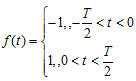
\includegraphics[width=0.15\textwidth]{cases.png}}

{} Si sabemos que:  
\[
a_{n}=\int_{-\frac{T}{2}}^{\frac{T}{2}}f(t)\cos(n\omega_{0}t)dt \hspace{10cm}
\]

\begin{figure}[h]
\centering
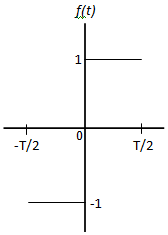
\includegraphics[width=0.15\textwidth]{ejemplo1.png}   
\caption{Ejemplo 1}
\label{fig:ejemplo1}
\end{figure}

{} Entonces:  
\[
a_{n}=\frac{2}{T}\left(\int_{-\frac{T}{2}}^{0}-\cos(n\omega_{0}t)dt+\int_{%
\frac{T}{2}}^{0}\cos(n\omega_{0}t)dt\right) \hspace{4cm}
\]
\[
=\frac{2}{T}\left(\left.-\frac{1}{n\omega_{0}}\sin(n\omega_{0}t)\right|_{-%
\frac{T}{2}}^{0} + \left.\frac{1}{n\omega_{0}}\sin(n\omega_{0}t)\right|_{0}^{%
\frac{T}{2}}\right) \hspace{3cm}
\]
\[
=\frac{T}{2}\left\{-\frac{1}{n\omega_{0}}[\sin(0)-\sin(n\pi)]-\frac{1}{%
n\omega_{0}}[\sin(n\pi)-\sin(0)] \right\}=0 \hspace{1.1cm}
\]
\[
b_{n}=\frac{T}{2}\left(\int_{-\frac{T}{2}}^{0}-\sin(n\omega_{0}t)dt+\int_{%
\frac{T}{2}}^{0}\sin(n\omega_{0}t)dt\right) \hspace{3.8cm}
\]
\newline

{} Si $n$ es par entonces es igual a $0$ 

{} Si $n$ es impar entonces sabemos que $\omega_0=\frac{2\pi}{T}$

\[
\frac{1}{n\pi}\left[2-(-1-1)\right]=\frac{4}{n(impar)\pi} \hspace{6.2cm}
\]
\newline
$f(x)$ = $\cases{\frac{4}{n\pi},& n impar \cr 0, & n par}$\newline
\vspace{0.5cm}

{} Entonces:  
\[
a_0=\frac{2}{T}\left[\int_{-\frac{T}{2}}^{0}+\int_{0}^{\frac{T}{2}}\right]=%
\frac{2}{T}\left[\left.t\right|_{-\frac{T}{2}}^{0}+  \left.t\right|_{0}^{%
\frac{T}{2}}\right] \hspace{8cm}
\]
\[
= \frac{2}{T}\left[\frac{T}{2}+0+0-\frac{T}{2}\right]=0 \hspace{9.3cm}
\]

{} En esta funci\'on $a_{n}=0$ y $a_{0}=0$ porque es una \textit{funci\'on
impar}.\newline

{} La serie de Fourier para esta funci\'on es:  
\[
f(t)=\sum_{n=impar}^{\infty}\frac{4}{n\pi}\sin\left(n\omega_{0}t\right)
\]

%%%%%%%%%%%%%%%%%%%%%%%%%%%%%%%%%%%%%%%%%%%%%%%%%%%%%%%%%%%%%%%%%%%%%%%%%%%%%%%%%%%%%%%%%%%%%%%%%%%%%%%%%%%%%%%%%%%%%%%%%%%%%%%%%%%%%%%%%%%%%%%%%%%%

\subsection{Determinaci\'on de la Serie de Fourier de Se\~nales El\'ectricas}

{} En algunos sistemas de telemetr\'ia es necesario producir una onda
sinusoidal con una frecuencia que est\'a relacionada con el voltaje de una
corriente de manera lineal. Por ejemplo, podemos necesitar que la salida de
un oscilador sea 370 Hz (hertz o ciclos por segundo). Cuando se apliquen 0
voltios de corriente directa (CD) y despu\'es que var\'{\i}\'ie linealmente
hasta 430 Hz cuando la entrada se eleve a 5 voltios de corriente directa. 

{} El problema es que la frecuencia de un oscilador de onda sinusoidal no
puede cambiarse mucho simplemente con una se\~{n}al el\'ectrica. Usualmente,
estos osciladores operan tomando una oscilaci\'on sinusoidal natural de otro
circuito inductor-capacitor o de un cristal, entonces (al girar la perilla
de sinton\'ia de un radio se est\'a cambiando el valor de un capacitor en un
circuito oscilador inductor-capacitor). Lo que se necesita en este caso es
la capacidad de cambiar la frecuencia de salida hasta en 7.5\% hacia
cualquier lado de la frecuencia fundamental utilizando \'unicamente una se%
\~{n}al el\'ectrica.

\begin{figure}[h]
\centering
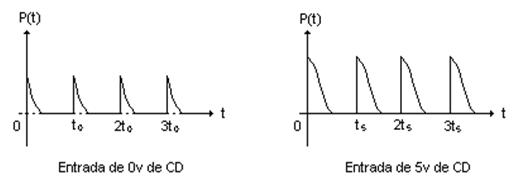
\includegraphics[width=0.50\textwidth]{senal.jpg}   
\caption{Salida de un generador de pulsos en 0v y 5v.}
\label{fig:senal}
\end{figure}

{} Estudiaremos ahora como se hace esto, empezaremos con un generador de
pulso capaz de producir pulsos peri\'odicamente (el mismo tiempo entre
pulsos) y con la capacidad adicional de poder cambiar significativamente
este periodo con un cambio en el voltaje de entrada. Esto es f\'acil de
hacer si no nos importa la forma de los pulsos. Ahora tomamos la salida del
generador de pulsos y la ponemos en un flip-flop con una salida que siempre
tiene uno de dos voltajes, digamos, $k$ y $-k$.

{} Si la salida es de $k$ voltios, se mantendr\'a as\'i hasta que reciba un
impulso de entrada. En este momento, cambia de estado y su salida cae a $-k$
voltios hasta que llegue el siguiente pulso. Como el tiempo entre los pulsos
es constante, la salida del flip-flop ser\'a una onda cuadrada de amplitud $k
$ y su frecuencia ser\'a de la mitad de la del generador de pulsos. Un
aumento en el voltaje en el generador de pulsos hace que aumente su
frecuencia, increment\'andose la frecuencia de la onda cuadrada. Por lo
tanto, es posible producir una onda cuadrada con una frecuencia que puede
cambiarse con un voltaje de entrada.

{} Lo que realmente se necesita es una onda sinusoidal con una frecuencia
que pueda cambiarse de esta manera. Como la onda cuadrada es peri\'odica y
satisface que en cada punto de un periodo las derivadas por la izquierda y
por la derecha existen (La serie de Fourier converge al promedio de los
limites izquierdo y derecho la funci\'on), sabemos que esta onda cuadrada es
una suma de ondas sinusoidales una de las cuales es la que queremos.

{} Supongamos que queremos una onda sinusoidal con frecuencia $\frac{\omega_0%
}{2\pi}$. Constituimos una onda cuadrada con frecuencia $\frac{\omega_0}{2\pi%
}$.La onda cuadrada de la salida de un Flip-Flop es: 

\begin{center}
%%%%%%%%%%%%%%Condicionalidades%%%%%%%%%%%%%%%%%%
$f(x)$ = $\cases{0<t<\frac{\pi}{\omega_0},& si k \cr
\frac{\pi}{\omega_0}<t<\frac{2\pi}{\omega_0}, & si -k}$  
%%%%%%%%%%%%%%Condicionalidades%%%%%%%%%%%%%%%%%%
\end{center}

\clearpage
\begin{figure}[h]
\centering{\  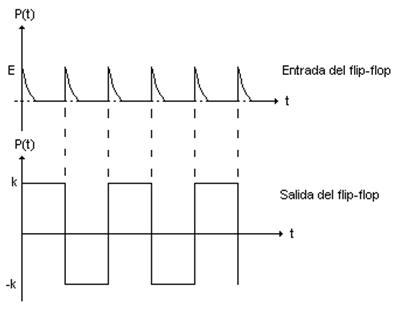
\includegraphics[width=0.40\textwidth]{flip_flop.jpg}}   
\caption{Flip-Flop}
\label{fig:flipflop}
\end{figure}

{} Y por tanto:  
\[
f\left[t+ \frac{2\pi}{\omega_0}\right]=f(t) \hspace{10cm}
\]

{} La serie de Fourier que representa la $f(t)$ es:\newline

{} Si sabemos que:  
\[
a_0=\frac{2}{T}\int_{-\frac{T}{2}}^{\frac{T}{2}}f(t)dt \hspace{9cm}
\]

{} Entonces tenemos:  
\[
a_0=\frac{2}{T}\left[\int_{0}^{\frac{\pi}{\omega}}kdt+\int_{\frac{\pi}{\omega%
}}^{\frac{2\pi}{\omega}}(-k)dt\right] \hspace{7cm}
\]
\[
=\frac{2}{T}\left[\left.kt\right|_{0}^{\frac{\pi}{\omega}}-\left.kt\right|_{%
\frac{\pi}{\omega}}^{\frac{2\pi}{\omega}}\right] \hspace{8cm}
\]
\[
=\frac{2}{T}\left[k\left(\frac{\pi}{\omega_0}-0\right)-k\left(\frac{2\pi}{%
\omega_0}-\frac{\pi}{\omega_0}\right)\right] \hspace{5.6cm}
\]
\[
=\frac{2}{T}\left[k\left(\frac{\pi}{\omega_0}\right)-k\frac{\pi}{\omega_0}%
\right] \hspace{7.7cm}
\]
\[
=\frac{2}{T}\left(0\right)=0 \hspace{9.3cm}
\]
\newline

{} Por lo tanto en coeficiente $a_0=0$ y sabiendo que:  
\[
a_n=\frac{2}{T}\int_{-\frac{T}{2}}^{\frac{T}{2}}f(t)\cos(n\omega_{0}t)dt
\]

{} Entonces:  
\[
a_n=\frac{2}{T}\left[\int_{0}^{\frac{\pi}{\omega}}k\cos(n\omega_{0}t)dt+
\int_{\frac{\pi}{\omega}}^{\frac{2\pi}{\omega}}(-k)\cos(n\omega_{0}t)dt%
\right] \hspace{5cm}
\]
\[
=\frac{2}{T}\left[\left.\frac{k}{n\omega_0}\sin(n\omega_{0}t)\right|_{0}^{%
\frac{\pi}{\omega}} - \left.\frac{k}{n\omega_{0}t}\sin(n\omega_{0}t)\right|_{%
\frac{\pi}{\omega}}^{\frac{2\pi}{\omega}}\right] \hspace{5.2cm}
\]
\[
=\frac{2}{T}\left[\frac{k}{n\omega_{0}}\left(\sin\left(n\omega_{0}\frac{n}{%
\omega_{0}}\right)-\sin(0)\right)- \frac{k}{n\omega_{0}}\left(\sin\left(n%
\omega_{0}t\frac{2\pi}{\omega_{0}}\right)-\sin\left(n\omega_{0}t\frac{\pi}{%
\omega_{0}}\right)\right)\right]
\]
\[
=\frac{2}{T}\left[\frac{k}{n\omega_{0}}\left(\sin(n\pi)-\sin(0)\right)- 
\frac{k}{n\omega_{0}}\left(\sin(n2\pi)-\sin(n\pi)\right)\right] \hspace{3.3cm%
}
\]
\[
=\frac{2}{T}\left[\frac{k}{n\omega_{0}}(0-0)-\frac{k}{n\omega_{0}}(0-0)%
\right] \hspace{7.1cm}
\]
\[
=\frac{2}{T}(0-0)=0 \hspace{9.7cm}
\]
\newline

{} Por lo tanto el coeficiente $a_n=0$  \newline

{} Si recordamos las propiedades de una funci\'on impar, notaremos que la
funci\'on que estamos analizando es una funci\'on impar, por eso los
coeficientes $a_n$ y $a_0$ son igual a cero.  \newline

{} Si sabemos que:  
\[
b_n=\frac{2}{T}\int_{-\frac{T}{2}}^{\frac{T}{2}}f(t)\sin(n\omega_{0}t)dt
\]

{} Entonces:  
\[
b_n=\frac{2}{T}\left[\int_{0}^{\frac{\pi}{\omega_{0}}}k\sin(n\omega_{0}t)dt+
\int_{\frac{\pi}{\omega_{0}}}^{\frac{2\pi}{\omega_{0}}}(-k)\sin(n%
\omega_{0}t)dt\right] \hspace{5.2cm}
\]
\[
=\frac{2}{T}\left[\left.-\frac{k}{n\omega_{0}}\cos(n\omega_{0}t)\right|_{0}^{%
\frac{\pi}{\omega_{0}}}+ \left.\frac{k}{n\omega_{0}}\cos(n\omega_{0}t)%
\right|_{\frac{\pi}{\omega_{0}}}^{\frac{2\pi}{\omega_{0}}}\right] \hspace{%
5.1cm}
\]
\[
=\frac{2}{T}\left[-\frac{k}{n\omega_{0}}\left(\cos\left(n\omega_{0}\frac{\pi%
}{\omega_{0}}\right)-\cos(0)\right)+ \frac{k}{n\omega_{0}}%
\left(\cos\left(n\omega_{0}\frac{2\pi}{\omega_{0}}\right)-\cos\left(n%
\omega_{0}\frac{\pi}{\omega_{0}}\right)\right)\right]
\]
\[
=\frac{2}{T}\left[-\frac{k}{n\omega_{0}}(\cos(n\pi)-\cos(0))+\frac{k}{%
n\omega_{0}}(\cos(n2\pi)-\cos(n\pi))\right] \hspace{3.3cm}
\]

{} Si $n$ es un n\'umero par, el $b_n=0$ y si $n$ es un n\'umero impar, con $%
\omega_{0}=\frac{2\pi}{T}$ entonces:  
\[
\frac{k}{n\pi}[2-(-1-1)]=\frac{4k}{n(impar)\pi}
\]

%%%%%%%%%%%%%%Condicionalidades%%%%%%%%%%%%%%%%%%
$b_n$ = $\cases{0,& n par \cr \frac{4k}{n\pi0}, & n impar}$  
%%%%%%%%%%%%%%Condicionalidades%%%%%%%%%%%%%%%%%%
\newline

{} La serie de Fourier que representa a $f(t)$ es:  
\[
f(t)=\frac{4k}{\pi}\sum_{n=1}^{\infty}\frac{\sin[(2n-1)\omega_{0}t]}{2n-1} 
\hspace{9.5cm}
\]
\[
=\frac{4k}{\pi}\sin(\omega_{0}t)+\frac{4k}{3\pi}\sin(3\omega_{0}t)+\frac{4k}{%
5\pi}\sin(5\omega_{0}t)+\ldots \hspace{5.1cm}
\]

{} Para los prop\'ositos actuales, solo queremos el primer t\'ermino
sinusoidal, de modo que eliminaremos las arm\'onicas m\'as altas colocando
la se\~{n}al de onda cuadrada en un filtro de frecuencias bajas. Este es
simplemente un circuito que permite el paso a frecuencias bajas
pr\'acticamente ilesas mientras que aten\'ua las frecuencias altas. Para ver
como se hace esto, consideraremos un ejemplo espec\'ifico. Supongamos que
queremos producir una onda sinusoidal de 400 hertzios y queremos cambiar
esta frecuencia el\'ectricamente desde 370 hertz hasta 430 hertz sin
distorsionar la se\~{n}al. Supondremos que el valor de la amplitud de salida
no es critica (dentro de l\'imites razonables); esto es cierto en la
pr\'actica. Lo que es crucial es la frecuencia de salida. 

{} Empezaremos con un generador de pulsos con una frecuencia que pueda
variar de 740 a 860 hertz con un cambio en la entrada de 0v a 5v de CD.
Hacemos una onda cuadrada poniendo estos pulsos en un flip-flop. La
frecuencia de la onda cuadrada ser\'a de la mitad de la del pulso del
generador y por lo tanto variara de 370 a 430 hertz. Ahora tenemos la onda
cuadrada superior con $\omega_{0}=800\pi$, esto es:

%%%%%%%%%%%%%%Condicionalidades%%%%%%%%%%%%%%%%%%

\begin{center}
$f(t)$ = $\cases{0<t<\frac{1}{800},& k \cr \cr
\frac{1}{800}<t<\frac{1}{400}, & -k}$ 
\end{center}

%%%%%%%%%%%%%%Condicionalidades%%%%%%%%%%%%%%%%%%	

{} Entonces:  
\[
f\left(t+\frac{1}{400}\right) \hspace{11cm}
\]

{} La funci\'on anterior tiene la siguiente serie de Fourier:  
\[
f(t)=\frac{4k}{\pi}\sum_{n=1}^{\infty}\frac{\sin[(2n-1)800\pi]}{2n-1} 
\hspace{9.5cm}
\]

{} Si tomamos esta se\~nal como entrada a un filtro pasa bajas \textit{%
inductor-capacitor}, debemos calcular $\frac{q(t)}{C}$; y a su vez debemos
conocer $q$.  
\begin{figure}[h]
\centering{\  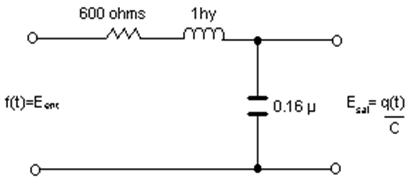
\includegraphics[width=0.50\textwidth]{circuito.jpg}}   
\caption{Circuito LRC}
\label{fig:circuito}
\end{figure}

{} La ecuaci\'on diferencial para este circuito es:  
\[
Li^{t}+Ri+\frac{q}{c}=f(t)
\]

{} Recordemos que $i=q^{t}$ y ponemos $f(t)$ y los valores de \textit{L, R y
C} en esta ecuaci\'on para obtener:  
\[
q^{tt}+600q^{t}+6.25(10^{6})q=\frac{4k}{\pi}\sum_{n=1}^{\infty}\frac{\sin[%
(2n-1)800\pi t]}{2n-1}
\]

{} Como queremos \'unicamente la soluci\'on estacionaria, desechamos la
soluci\'on homog\'enea y consideramos las ecuaciones diferenciales no
homoh\'eneas.  
\[
q^{tt}+600q^{t}+6.25(10^{6})q=\frac{4k}{\pi}\sin(800\pi t) \hspace{8cm}
\]
\[
q^{tt}+600q^{t}+6.25(10^{6})q=\frac{4k}{3\pi}\sin(2400\pi t) \hspace{7.8cm}
\]
\[
q^{tt}+600q^{t}+6.25(10^{6})q=\frac{4k}{5\pi}\sin(4000\pi t) \hspace{7.8cm}
\]

{} Hasta  
\[
q^{tt}+600q^{t}+6.25(10^{6})q=\frac{4k}{(2n-1)\pi}\sin[(2n-1)800\pi t] 
\hspace{5.7cm}
\]

{} La estrategia es resolver cada una de estas ecuaciones diferenciales y
sumar las soluciones para encontrar la representaci\'on en serie de Fourier
de la carga del capacitor $q$. As\'i consideramos:  
\[
q_{n}^{tt}+600q_{n}^{t}+6.25(10^{6})q_{n}=\frac{4k}{n\pi}\sin(n\omega_{0} t) 
\hspace{7.8cm}
\]

{} Donde $n$ es cualquier n\'umero positivo impar y $\omega_{0}=800\pi$. El
sub\'indice $n$ se introduce para recordarnos que esta es la en\'esima
ecuaci\'on y debemos sumar las soluciones.

%%%%%%%%%%%%%%%%%%%%%%%%%%%%%%%%%%%%%%%%%%%%%%%%%%%%%%%%%%%%%%%%%%%%%%%%%%%%%%%%%%%%%%%%%%%%%%%%%%%%%%%%%%%%%%%%%%%%%%%%%%%%%%%%%%%%%%%%%%%%%%%%%%%%

\subsection{Interpretaci\'on Geom\'etrica de la serie de Fourier}

\subsubsection{Condiciones de Dirichlet}

{} Se supuso que las funciones dadas se pod\'ian interpretar mediante una
serie de Fourier. Pero ahora se debe investigar la convergencia de la serie
de Fourier de una funci\'on $f(t)$. 

{} El argumento que motiva la definici\'on de los coeficientes de Fourier
depend\'ia de poder intercambiar una serie con una integral, un paso que en
general no es v\'alido. Se tendr\'a que saber las condiciones sobre $f(t)$
que nos permitan determinar la suma de la serie de Fourier de $f(t)$ en un
intervalo. \newline

{} Recordemos que $f(t)$ es continua en pedazos si: 

\begin{enumerate}
\item $\lim_{x\to a^{+}}f(x)$ y $\lim_{x\to a^{-}}f(x)$ son finitos. 

\item $f(t)$ es continua en todos sus puntos de $[a,b]$ excepto posiblemente
un n\'umero finito de ellos. 

\item En los puntos $(a,b)$ donde $f(t)$ es discontinua, la funci\'on tiene
l\'imite izquierdo y derecho finitos. 
\end{enumerate}

{} La siguiente figura muestra la gr\'afica de una funci\'on que es continua
a pedazos. En los puntos de $(a,b)$ donde la funci\'on es discontinua, la
gr\'afica tiene discontinuidades de salto. La magnitud del salto en $x_{0}$
es la diferencia entre el l\'imite izquierdo y derecho en ese punto:  
\[
\left|\lim_{h\to 0^{+}}f(x_{0}+h)-\lim_{h\to 0^{-}}f(x_{0}+h)\right|
\]

{} Esta es la distancia entre el extremo izquierdo y derecho de la gr\'afica
en $x_{0}$.  
\begin{figure}[h]
\centering{\  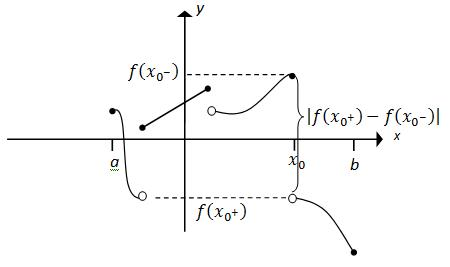
\includegraphics[width=0.50\textwidth]{limites.jpg}}   
\caption{Condiciones Dirichlet}
\label{fig:limite}
\end{figure}

{} Se denotan el limite izquierdo y derecho de la siguiente manera:  
\[
f(x_{0^{+}})=\lim_{k\to 0^{+}}f(x_{0}+h) \hspace{3cm} f(x_{0^{-}})=\lim_{k%
\to 0^{-}}f(x_{0}+h) 
\]

{} Si estos l\'imites existen y son finitos, tambi\'en existen las derivadas
tanto por la izquierda como por la derecha aunque la derivada de la
funci\'on no exista. 

{} Se enunciar\'an aqu\'i las condiciones, conocidas como \textit{%
Condiciones de Dirichlet}, baja las cuales es posible la representaci\'on en
serie de Fourier de una funci\'on dada $f(t)$. 

\begin{enumerate}
\item La funci\'{o}n $f(t)$ tiene un n\'umero finito de discontinuidades en
un periodo. 

\item La funci\'{o}n $f(t)$ tiene un n\'umero finito de m\'aximos y
m\'inimos en un periodo. 

\item La integral del valor absoluto de $f(t)$ en un periodo es finita, es
decir:  
\[
\int_{-\frac{t}{2}}^{\frac{t}{2}}|f(t)|dt=finita<\infty
\]
\end{enumerate}

{} Se dice que una funci\'on $f(t)$ es continua por tramos en el intervalo
finito $\left[-\frac{t}{2},\frac{t}{2}\right]$ si satisface las condiciones $%
1$. y $2$.

{} Si $a_n$ y $b_n$ son las sucesiones de los coeficientes de $f(t)$,
entonces:  
\[
\lim_{n\to \infty}a_{n}=\lim_{n\to \infty}b_{n}=0
\]

{} Y si se tiene que:  
\[
\frac{1}{2}a_{0}^{2}+\sum_{n=1}^{\infty}\left(a_{n}^{2}+b_{n}^{2}\right)\leq 
\frac{2}{T}\int_{-\frac{T}{2}}^{\frac{T}{2}}|f(t)|^{2}dt
\]

{} Puesto que la serie del miembro izquierdo es convergente entonces es
necesario que:  
\[
\lim_{n\to \infty}\left(a_{n}^{2}+b_{n}^{2}\right)=0
\]

{} Lo cual implica que:  
\[
\lim_{n\to \infty}a_{n}=\lim_{n\to \infty}b_{n}=0
\]

{} \textbf{Ejemplo:} 

{} Demostrar que si $f(t)$ es una funci\'on continua por tramos, la integral
del valor absoluto de $f(t)$ es finita en el intervalo $-\frac{T}{2}<t<\frac{%
T}{2}$, entonces:  
\[
\lim_{n\to \infty}\int_{-\frac{T}{2}}^{\frac{T}{2}}f(t)\cos(n\omega_{0}t)dt=
\lim_{n\to \infty}\int_{-\frac{T}{2}}^{\frac{T}{2}}f(t)\sin(n\omega_{0}t)dt=
0
\]

{} Los coeficientes de Fourier existen, puesto que la integral del valor
absoluto de $f(t)$ es finita en el intervalo $[\frac{T}{2},-\frac{T}{2}]$  
%%%%%%%%%%%%%%Condicionalidades%%%%%%%%%%%%%%%%%%
\[
\lim_{n\to \infty} \cases{a_{n} \cr \cr b_{n}}= \lim_{n\to \infty}\frac{2}{T}%
\int_{-\frac{T}{2}}^{\frac{T}{2}}f(t) \cases{\cos(n\omega_{0}t) \cr \cr
\sin(n\omega_{0}t)}dt=0
\]
%%%%%%%%%%%%%%Condicionalidades%%%%%%%%%%%%%%%%%%	

%%%%%%%%%%%%%%%%%%%%%%%%%%%%%%%%%%%%%%%%%%%%%%%%%%%%%%%%%%%%%%%%%%%%%%%%%%%%%%%%%%%%%%%%%%%%%%%%%%%%%%%%%%%%%%%%%%%%%%%%%%%%%%%%%%%%%%%%%%%%%%%%%%%%

\subsection{Serie de Fourier Compleja}

{} La representaci\'on de una funci\'on peri\'odica como una serie de
Fourier, implica que la especificaci\'on de sus coeficientes determina
un\'ivocamente la funci\'on. Ahora desarrollaremos la forma compleja de la
serie de Fourier que nos proveer\'a de un contexto natural desde el cual
podemos considerar muchos resultados del an\'alisis de Fourier incluyendo la
transformada de Fourier.

\subsubsection{Definici\'on de la Serie de Fourier Compleja}

{} En muchas aplicaciones de las series de Fourier, es conveniente expresar
estas series en t\'erminos de los exponenciales complejos $e^{\pm
jn\omega_{0}t}$ 

{} Si se considera la serie de Fourier de una funci\'on peri\'odica $(t)$,
como:  
\[
f(t)=\frac{1}{2}a_{0}+\sum_{n=1}^{\infty}\left(a_{n}\cos(n\omega_{0}t)+b_{n}%
\sin(n\omega_{0}t)\right)
\]

{} Donde $\omega_{0}=\frac{2\pi}{T}$, el seno y el coseno se pueden expresar
en t\'erminos de los exponenciales como:  
\[
\cos(n\omega_{0}t)=\frac{1}{2}\left(e^{jn\omega_{0}t}+e^{-jn\omega_{0}t}%
\right)
\]
\[
\sin(n\omega_{0}t)=\frac{1}{2}\left(e^{jn\omega_{0}t}-e^{-jn\omega_{0}t}%
\right)
\]

{} Sustituyendo esto en la serie de Fourier, tenemos:  
\[
f(t)=\frac{1}{2}a_{0}+\sum_{n=1}^{\infty}\left(a_{n}\frac{1}{2}%
\left(e^{jn\omega_{0}t}+e^{-jn\omega_{0}t}\right) +b_{n}\frac{1}{2}%
\left(e^{jn\omega_{0}t}-e^{-jn\omega_{0}t}\right)\right)
\]

{} Teniendo en cuenta que $\frac{1}{j}=-j$, se puede expresar como:  
\[
f(t)=\frac{1}{2}a_{0}+\sum_{n=1}^{\infty}\left(\frac{1}{2}%
\left(a_{n}-jb_{n}\right)e^{jn\omega_{0}t} +\frac{1}{2}\left(a_{n}+jb_{n}%
\right)e^{-jn\omega_{0}t}\right)
\]

{} Si se hace:  
\[
c_{0}=\frac{1}{2}a_{0} \hspace{12.6cm}
\]
\[
c_{n}=\frac{1}{2}(a_{n}-jb_{n}) \hspace{11.3cm}
\]
\[
c_{-n}=\frac{1}{2}(a_{n}+jb_{n}) \hspace{11cm}
\]

{} Entonces:  
\[
f(t)=c_{0}+\sum_{n=1}^{\infty}\left(\frac{1}{2}c_{n}e^{jn\omega_{0}t} +\frac{%
1}{2}c_{-n}e^{-jn\omega_{0}t}\right) \hspace{7.2cm}
\]
\[
=c_{0}+\sum_{n=1}^{\infty}\frac{1}{2}c_{n}e^{jn\omega_{0}t}+\sum_{n=-1}^{-%
\infty}\frac{1}{2}c_{n}e^{jn\omega_{0}t} \hspace{6.6cm}
\]
\[
=\sum_{-\infty}^{\infty}\frac{1}{2}c_{n}e^{jn\omega_{0}t} \hspace{10cm}
\]

{} A esta ecuaci\'on se le denomina serie compleja de Fourier de $f(t)$. Y a
los coeficientes $c_{n}$ se pueden evaluar f\'acilmente en t\'erminos de $%
a_{n}$ y $b_{n}.$  
\[
c_{0}=\frac{1}{2}a_{0}=\frac{1}{T}\int_{-\frac{T}{2}}^{\frac{T}{2}}f(t)dt
\]

\[
c_{n}=\frac{1}{2}(a_{n}-jb_{n}) \hspace{10.5cm}
\]
\[
=\frac{1}{T}\left[\int_{-\frac{T}{2}}^{\frac{T}{2}}f(t)\cos(n\omega_{0}t)dt
-j\int_{-\frac{T}{2}}^{\frac{T}{2}}f(t)\sin(n\omega_{0}t)dt\right] \hspace{%
4.1cm}
\]
\[
=\frac{1}{T}\left[\int_{-\frac{T}{2}}^{\frac{T}{2}}f(t)\left(\cos(n%
\omega_{0}t)dt -j\sin(n\omega_{0}t)\right)dt\right] \hspace{5.1cm}
\]
\[
=\frac{1}{T}\int_{-\frac{T}{2}}^{\frac{T}{2}}f(t)e^{-jn\omega_{0}t}dt 
\hspace{8.6cm}
\]
\[
c_{-n}=\frac{1}{2}(a_{n}-jb_{n})=\frac{1}{T}\int_{-\frac{T}{2}}^{\frac{T}{2}%
}f(t)e^{jn\omega_{0}t}dt \hspace{7.1cm}
\]

{} Si $f(t)$ es real, $c_{-n}=c_{n}^{*}$, donde '$*$' indica el campo
conjugado, entonces tenemos:  
\[
f(t)=c_{0}+\sum_{n=1}^{\infty}\left(\frac{1}{2}c_{n}e^{jn\omega_{0}t}+ \frac{%
1}{2}c_{-n}e^{-jn\omega_{0}t}\right) \hspace{6.5cm}
\]
\[
=c_{0}+\sum_{n=1}^{\infty}\frac{1}{2}c_{n}e^{jn\omega_{0}t}+\sum_{n=-1}^{-%
\infty}\frac{1}{2}c_{n}e^{jn\omega_{0}t} \hspace{6cm}
\]
\[
=\sum_{-\infty}^{\infty}\frac{1}{2}c_{n}e^{jn\omega_{0}t} \hspace{9.5cm}
\]

{} A esta ecuaci\'on se le denomina \textit{Serie Compleja de Fourier} de $%
f(t)$.

%%%%%%%%%%%%%%%%%%%%%%%%%%%%%%%%%%%%%%%%%%%%%%%%%%%%%%%%%%%%%%%%%%%%%%%%%%%%%%%%%%%%%%%%%%%%%%%%%%%%%%%%%%%%%%%%%%%%%%

\subsubsection{Determinaci\'on de la Serie Compleja de Se\~{n}ales}

{} Determinaremos la serie de Fourier compleja de la funci\'on serrucho $f$
de periodo 8 definida por:  
\[
f(t)=\frac{3}{4}t \hspace{1cm} para \hspace{1cm} 0<t<8
\]
\[
f(t+8)=f(t) \hspace{3.2cm}
\]

\begin{figure}[h]
\centering{\  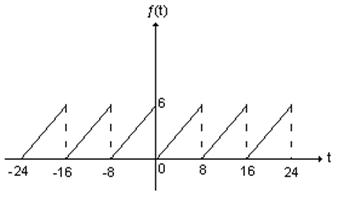
\includegraphics[width=0.40\textwidth]{grafica_scsenales.jpg}}
\caption{Serie de Fourier Compleja}
\label{fig:seriecompleja}
\end{figure}

{} Aqu\'i tenemos $T=8$ y $\omega_{0}=\frac{2\pi}{8}=\frac{\pi}{4}$ si $%
n\neq 0$. Si sabemos que la serie compleja de Fourier es:  
\[
f(t)=c_{0}+\sum_{n=-\infty}^{\infty}c_{n}e^{jn\omega_{0}t}
\]

{} Con:  
\[
c_{0}=\frac{1}{T}\int_{-\frac{T}{2}}^{\frac{T}{2}}f(t)dt \hspace{2cm} c_{n}=%
\frac{1}{T}\int_{-\frac{T}{2}}^{\frac{T}{2}}f(t)e^{-jn\omega_{0}t}dt
\]

{} Entonces:  
\[
c_{n}=\frac{1}{T}\int_{-\frac{T}{2}}^{\frac{T}{2}}f(t)e^{-jn\omega_{0}t}dt 
\hspace{10cm}
\]
\[
= \frac{1}{8}\int_{-\frac{8}{2}}^{\frac{8}{2}}\frac{3}{4}te^{-jn%
\omega_{0}t}dt=\frac{3}{32}\int_{0}^{8}te^{-jn\omega_{0}t}dt \hspace{6.8cm}
\]
\[
u=t \hspace{1cm} du=dt \hspace{9.2cm}
\]
\[
v=\frac{e^{-jn\omega_{0}t}}{-jn\omega_{0}} \hspace{1cm} dv=e^{-jn%
\omega_{0}t}dt \hspace{7cm}
\]

{} Entonces:  
\[
=\frac{3}{32}\left[t\frac{e^{-jn\omega_{0}t}}{-jn\omega_{0}}-\int_{0}^{8}%
\frac{e^{-jn\omega_{0}t}}{-jn\omega_{0}}dt\right]_{0}^{8} \hspace{7.8cm}
\]
\[
=\frac{3}{32}\left[t\frac{e^{-jn\omega_{0}t}}{-jn\omega_{0}}-\frac{%
e^{-jn\omega_{0}t}}{\left(-jn\omega_{0}\right)^{2}}\right]_{0}^{8} \hspace{%
8.3cm}
\]

{} Si:  
\[
\omega_{0}=\frac{2\pi}{8}=\frac{\pi}{4} \hspace{14cm}
\]
%pag 23
%%%%%%%%%%%%%%%%%%%%%%%%%%%%%%%%%%%%%%%%%%%%%%%%%%%%%%%%%%%%%%%%%%%%%%%%%%%%%%%%%%%%%%%%%%%%%%%%%%%%%%%%%%%%%%%%%%%%%%%%%%%%%%%%%%%%%%%%%%%%%%%%%%%%
\clearpage{} {} {} 
%%%%%%%%%%%%%%%%%%%%%%%%%%%%%%%%%%%%%%%%%%%%%%%%%%%%%%%%%%%%%%%%%%%%%%%%%%%%%%%%%%%%%%%%%%%%%%%%%%%%%%%%%%%%%%%%%%%%%%%%%%%%%%%%%%%%%%%%%%%%%%%%%%%%

\end{document}
